\documentclass[]{article}

% Imports the catppuccin theme, using the mocha flavor,
% from the directory above. Actual implementation
% wouldn't need the import package unless the theme
% and the document are in different directories.
\usepackage{import}
\usepackage{xcolor}
\usepackage{cancel}
\usepackage{mathtools}
\usepackage{venndiagram}

% For permutations and combinations
\newcommand\Myperm[2][^n]{\prescript{#1\mkern-2.5mu}{}P_{#2}}
\newcommand\Mycomb[2]{\prescript{#1\mkern-0.5mu}{}C_{#2}}

% Colors
\definecolor{yorhabg}{HTML}{FFFFFF}
\definecolor{yorhafg}{HTML}{000000}
\definecolor{yorhagrid}{HTML}{B5AF9C}
\definecolor{mred}{HTML}{D67069}
\definecolor{mblue}{HTML}{6887A1}

\pagecolor{yorhabg}
\color{yorhafg}

\usepackage{preamble}

% Removes padding above title
\usepackage{titling}
\setlength{\droptitle}{-10em}

% Font package
\usepackage[T1]{fontenc}

\usepackage{fouriernc}

\usepackage{sectsty}
\usepackage{graphicx}
\usepackage{amsmath}
\usepackage{amsfonts}
\usepackage{amssymb}
\usepackage[skins, most]{tcolorbox}

\DeclareMathOperator{\sgn}{sgn}

\usepackage{tikz}
\usepackage{eso-pic}
\usetikzlibrary{calc,shadows.blur}
\usetikzlibrary{angles, quotes}
\usetikzlibrary{3d}

% Margins
\topmargin=0in
\evensidemargin=0in
\oddsidemargin=0in
\textwidth=6.5in
\textheight=9.0in
\headsep=0.25in

\AtBeginEnvironment{tcolorbox}{\small}

\newtcolorbox{imp}{enhanced,arc=0mm,colback=yorhabg,colframe=mred,leftrule=10mm,coltext=yorhafg,%
overlay={\node[anchor=west,outer sep=2pt] at (frame.west) {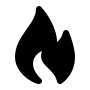
\includegraphics[width=6mm]{images/imageb.png}}; }}

\newtcolorbox{shortcut}{enhanced,arc=0mm,colback=yorhabg,colframe=mred,leftrule=10mm,coltext=yorhafg, coltitle=yorhabg, title=\texttt{Shortcut.}, 
overlay={\node[anchor=west,outer sep=2pt] at (frame.west) {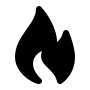
\includegraphics[width=6mm]{images/imageb.png}}; }}

\newtcolorbox{question}{
    enhanced, 
    colback=yorhabg,
    colframe=mblue,
    coltext=yorhafg,
    coltitle=yorhabg,
    attach boxed title to top left={yshift*=-\tcboxedtitleheight}, 
    title=\texttt{Question.},
    boxed title size=title,
    boxed title style={%
        rounded corners=northeast, 
        rounded corners=northwest, 
        colback=tcbcolframe, 
        boxrule=0pt,
    },
    underlay boxed title={%
        \path[fill=tcbcolframe] (title.south west)--(title.south east) 
            to[out=0, in=180] ([xshift=5mm]title.east)--
            (title.center-|frame.east)
            [rounded corners=5pt] |- 
            (frame.north) -| cycle; 
    },
}

\newcommand\bb[1]{\textcolor{yorhafg}{\textbf{#1}}}

\title{\textbf{CSCA67 - Exercises \#3}}
\author{ Satyajit Datta }
\date{\today}

\begin{document}

\maketitle    

\section*{1. Conditionals}

Analyse the logical forms of the following statements. Construct a converse and a contrapositive for
each conditional statement: provide your answers both as logical expressions and English sentences.
\hrule
\vspace{0.1in}
1. If Alice is at the party, then so is Bob.
\begin{align*}
    \text{Converse: } & B \rightarrow A 
        && \text{(If Bob is at the party, then so is Alice.)} \\
    \text{Contrapositive: } & \neg B \rightarrow \neg A 
        && \text{(If Bob is not at the party, then Alice is not at the party.)}
\end{align*}

2. Charlie is at the party, only if both Alice and Bob are.
\begin{align*}
    \text{Original: } & C \rightarrow (A \land B) \\
    \text{Converse: } & (A \land B) \rightarrow C 
        && \text{(Alice and Bob are both at the party, only if Charlie is.)} \\
    \text{Contrapositive: } & \neg (A \land B) \rightarrow \neg C 
        && \text{(If both Alice and Bob are not at the party, then Charlie is not at the party.)}
\end{align*}

3. David is not at the party, if Alice is.
\begin{align*}
    \text{Original: } & A \rightarrow \neg D \\
    \text{Converse: } & \neg D \rightarrow A
        && \text{(If David is not at the party, then Alice is.)} \\
    \text{Contrapositive: } & D \rightarrow \neg A
        && \text{(If David is at the party, then Alice is not.)}
\end{align*}

4. If Bob is not at the party, then Alice is.
\begin{align*}
    \text{Original: } & \neg B \rightarrow A \\
    \text{Converse: } & A \rightarrow \neg B
        && \text{(If Alice is at the party, the Bob is not.)} \\
    \text{Contrapositive: } & \neg A \rightarrow B
        && \text{(If Alice is not at the party, then Bob is.)}
\end{align*}

5. If Bob is not at the party, then neither is Alice.
\begin{align*}
    \text{Original: } & \neg B \rightarrow \neg A \\
    \text{Converse: } & \neg A \rightarrow \neg B
        && \text{(If Alice is not at the party, then neither is Bob.)} \\
    \text{Contrapositive: } & A \rightarrow B
        && \text{(If Alice is at the party, then so is Bob.)}
\end{align*}

6. Alice is not at the party, unless Bob is.
\begin{align*}
    \text{Original: } & A \rightarrow B \\
    \text{Converse: } & B \rightarrow A
        && \text{(If Bob is at the party, then Alice is.)} \\
    \text{Contrapositive: } & \neg B \rightarrow \neg A
        && \text{(If Bob is not at the party, then neither is Alice.)}
\end{align*}

7. Neither Alice nor Bob being at the party is a sufficient condition for Charlie to be at the party.
\begin{align*}
    \text{Original: } & \neg(A \land B) \rightarrow C \\
    \text{Converse: } & C \rightarrow \neg(A \land B)
        && \text{(If Charlie is at the party, then neither Alice nor Bob is.)} \\
    \text{Contrapositive: } & \neg C \rightarrow (A \land B)
        && \text{(If Charlie is not at the party, then both Alice and Bob are.)}
\end{align*}

8. Both Alice and Bob being at the party is a necessary condition for Charlie to be at the party.
\begin{align*}
    \text{Original: } & C \rightarrow (A \land B) \\
    \text{Converse: } & (A \land B) \rightarrow C
        && \text{(If both Alice and Bob is at the party, then so is Charlie.)} \\
    \text{Contrapositive: } & \neg(A \land B) \rightarrow \neg C
        && \text{(If both Alice and Bob are not at the party, then neither is Charlie.)}
\end{align*}

\section*{2. Logical Equivalences}
For each pair of expressions, either prove that the two are equivalent or prove that they are not.
\hrule
\vspace{0.1in}

1. $\neg(a \rightarrow b)$ and $\neg a \land b$

\begin{center}
\text{When } a \text{ is True, and } b \text{ is False, then:}
\end{center}
\begin{align*}
    \neg(a \rightarrow b) && \neg a \land b \\
    \Rightarrow \neg(T \rightarrow F) && \Rightarrow \neg T \land F \\
    \Rightarrow \neg(F) && \Rightarrow F \land F \\
    \Rightarrow T && \Rightarrow F
\end{align*}
\begin{center}
    $\therefore$ \text{The statements are not equivalent.} $\blacksquare$
\end{center}

2. $\neg(a \rightarrow b)$ and $a \land \neg b$
\begin{align*}
    \neg(a \rightarrow b) &&&& \boxed{a \land \neg b} \\
    \Rightarrow \neg(\neg a \land b) && \text{(Conditional Law)}  \\
    \Rightarrow \neg\neg a \lor \neg b && \text{(De Morgan's Law)} \\
    \Rightarrow \boxed{a \lor \neg b} &&\text{(Double Negation Law)} \\
\end{align*}
\begin{center}
    $\therefore$ The statements are equivalent. $\blacksquare$
\end{center}

3. $a \iff \neg b$ and $(a \land \neg b) \lor (\neg a \land b)$
\begin{align*}
    a \iff \neg b &&&& \boxed{(a \land \neg b) \lor (\neg a \land b)} \\
    \Rightarrow (\neg b \rightarrow a) \land (a \rightarrow \neg b) && \text{(Biconditional Law)} \\
    \Rightarrow (\neg\neg b \lor a) \land (\neg a \lor \neg b)   && \text{(Conditional Law)} \\
    \Rightarrow (b \lor a) \land (\neg a \lor \neg b) && \text{(Double Negation Law)} \\
    \Rightarrow ((b \lor a) \land \neg a) \lor ((b \lor a) \land \neg b) && \text{(Distributive Law)} \\
    \Rightarrow ((b \land \neg a) \lor (a \land \neg a)) \lor ((b \land \neg b) \lor (a \land \neg b)) && \text{(Distributive Law)} \\
    \Rightarrow \boxed{(b \land \neg a) \lor (a \land \neg b)} && \text{(Negation Law)}
\end{align*}
\begin{center}
    $\therefore$ The statements are equivalent. $\blacksquare$
\end{center}

\section*{3. Logical Inference}
Use the rules of inference from class, to prove validity of the following arguments.
\hrule
\vspace{0.1in}
1. If I play hockey, then I am sore the next day. I use the whirlpool if I am sore. I did not use
the whirlpool. Therefore, I did not play hockey.
\[
    \text{Statements} = 
    \begin{cases*}
         H: \text{I played hockey.} \\
         S: \text{I am sore the next day.} \\
         W: \text{I used the whirlpool.}
    \end{cases*}
\]

The argument is:

\begin{align*}
    & H \rightarrow S & (1)\\
    & S \rightarrow W & (2)\\
    & \neg W  & (3) \\
    & \overline{\therefore \neg H} & \text{Conclusion}
\end{align*}
New statements that we can make are:
\begin{align*}
    \neg S \quad & \text{(3), (2), Modus Tollens} \hfill & (4) \\
    \neg H \quad & \text{(4), (1), Modus Tollens} \hfill & (5) \\
\end{align*}

\begin{center}
    (5) $\equiv$ Conclusion, therefore the argument is true. $\blacksquare$
\end{center}
\hrule
\vspace{0.1in}
2. I am either dreaming or hallucinating. I am not dreaming. If I am hallucinating, I see elephants
running down the road. Therefore, I see elephants running down the road.
\[
    \text{Statements} = 
    \begin{cases*}
         D: \text{I am dreaming.} \\
         H: \text{I am hallucinating} \\
         E: \text{I see elephants running down the road.}
    \end{cases*}
\]

The argument is:

\begin{align*}
    & D \lor H & (1)\\
    & \neg D & (2)\\
    & H \rightarrow E  & (3) \\
    & \overline{\therefore  E} & \text{Conclusion}
\end{align*}
New statements that we can make are:
\begin{align*}
    H \quad & \text{(2), (1), Disjunctive Syllogism} \hfill & (4) \\
    E \quad & \text{(4), (3), Modus Ponens} \hfill & (5) \\
\end{align*}

\begin{center}
    (5) $\equiv$ Conclusion, therefore the argument is true. $\blacksquare$
\end{center}
\hrule
\vspace{0.1in}
3. If I go running, I stay in the sun for too long. If I go swimming, I stay in the sun for too long.
If I stay in the sun for too long, I get sunburn. I did not get a sunburn. Therefore, I neither
went running nor swimming.\[
    \text{Statements} = 
    \begin{cases*}
         R: \text{I went running.} \\
         S: \text{I stay in the sun for too long.} \\
         W: \text{I went swmming.}\\
         B: \text{I get sunburn.}
    \end{cases*}
\]

The argument is:

\begin{align*}
    & R \rightarrow S & (1)\\
    & W \rightarrow S & (2)\\
    & S \rightarrow B  & (3) \\
    & \neg B & (4) \\
    & \overline{\therefore (\neg R \land \neg W)} & \text{Conclusion}
\end{align*}
New statements that we can make are:
\begin{align*}
    \neg S \quad & \text{(3), (4), Modus Tollens} \hfill & (5) \\
    \neg W \quad & \text{(5), (2), Modus Tollens} \hfill & (6) \\
    \neg R \quad & \text{(5), (1), Modus Tollens} \hfill & (7) \\
    \neg R \land \neg W \quad & \text{(6), (7), Conjunction} \hfill & (8)
\end{align*}

\begin{center}
    (8) $\equiv$ Conclusion, therefore the argument is true. $\blacksquare$
\end{center}

\section*{4. Variables and Sets}

If $U$ is the universe of discourse, then the complement of the set $A$, which we will denote as A, is the set 
$$U \text{\textbackslash} A = \{x \in U \mid x \notin A\}$$
Use Venn diagrams to illustrate the following identities.
\vspace{0.1in}
\hrule
\vspace{0.1in}
1. $\overline{A \cup B} = \overline{A} \cap \overline{B}$


\[
\begin{tabular}{{c@{\hspace{1.5cm}}|@{\hspace{1.5cm}}c
}}
    $\mathbf{\overline{A \cup B}}$ & $\mathbf{\overline{A} \cap \overline{B}}$ \\
    \\
    \begin{venndiagram2sets}[tikzoptions={scale=0.8,thick}]
        \fillA
    \end{venndiagram2sets} 
    &
    \begin{venndiagram2sets}[tikzoptions={scale=0.8,thick}]
        \fillNotA
    \end{venndiagram2sets} 
    \\
    $A$ & $\overline{A}$ \\[1.5cm]
    \begin{venndiagram2sets}[tikzoptions={scale=0.8,thick}]
        \fillB
    \end{venndiagram2sets}
    &
    \begin{venndiagram2sets}[tikzoptions={scale=0.8,thick}]
        \fillNotB
    \end{venndiagram2sets} \\
    $B$ & $\overline{B}$ \\[1.5cm]
    \begin{venndiagram2sets}[tikzoptions={scale=0.8,thick}]
        \fillA
        \fillB
    \end{venndiagram2sets}
    &
    \begin{venndiagram2sets}[tikzoptions={scale=0.8,thick}]
        \fillNotAorB
    \end{venndiagram2sets} \\
    $ A \cup B$ & $\overline{A} \cap \overline{B}$ \\[1.5cm]
    \begin{venndiagram2sets}[tikzoptions={scale=0.8,thick}]
        \fillNotAorB
    \end{venndiagram2sets} \\
    $\overline{A \cup B}$ & \fbox{$\therefore \overline{A \cup B} = \overline{A} \cap \overline{B}$}\\
    
\end{tabular}
\]

2. $\overline{A \cap B} = \overline{A} \cup \overline{B}$


\[
\begin{tabular}{{c@{\hspace{1.5cm}}|@{\hspace{1.5cm}}c
}}
    $\mathbf{\overline{A \cap B}}$ & $\mathbf{\overline{A} \cup \overline{B}}$ \\
    \\
    \begin{venndiagram2sets}[tikzoptions={scale=0.8,thick}]
        \fillA
    \end{venndiagram2sets} 
    &
    \begin{venndiagram2sets}[tikzoptions={scale=0.8,thick}]
        \fillNotA
    \end{venndiagram2sets} 
    \\
    $A$ & $\overline{A}$ \\[1.5cm]
    \begin{venndiagram2sets}[tikzoptions={scale=0.8,thick}]
        \fillB
    \end{venndiagram2sets}
    &
    \begin{venndiagram2sets}[tikzoptions={scale=0.8,thick}]
        \fillNotB
    \end{venndiagram2sets} \\
    $B$ & $\overline{B}$ \\[1.5cm]
    \begin{venndiagram2sets}[tikzoptions={scale=0.8,thick}]
        \fillACapB
    \end{venndiagram2sets}
    &
    \begin{venndiagram2sets}[tikzoptions={scale=0.8,thick}]
        \fillNotAorB
        \fillANotB
        \fillBNotA
    \end{venndiagram2sets} \\
    $ A \cap B$ & $\overline{A} \cup \overline{B}$ \\[1.5cm]
    \begin{venndiagram2sets}[tikzoptions={scale=0.8,thick}]
        \fillNotAorB
        \fillANotB
        \fillBNotA
    \end{venndiagram2sets} \\
    $\overline{A \cap B}$ & \fbox{$\therefore \overline{A \cap B} = \overline{A} \cup \overline{B}$}\\
    
\end{tabular}
\]

\vspace{1.2in}
Prove the identities in part (a), by writing out (using logical symbols) what it means for anobject x to be an element of each set and then using logical equivalences.
\vspace{0.1in}
\hrule
\vspace{0.1in}
1. $\overline{A \cup B} = \overline{A} \cap \overline{B}$

\[
\begin{tabular}{{c@{\hspace{1.5cm}}|@{\hspace{1.5cm}}c
}}
    $\mathbf{\overline{A \cup B}}$ & $\mathbf{\overline{A} \cap \overline{B}}$ \\
    \\
    $\{x \text{\textbar} x \in (\overline{A \cup B})\}$ & $x \in \overline{A} \cap \overline{B}$ \\
        $\{x \text{\textbar} x \in \overline{A \cup B}\}$ & $\Rightarrow x \in \overline{A} \land x \in \overline{B}$ \\
    $\Rightarrow x \notin A \land x \notin B$ & $\Rightarrow x \notin A \land x \notin B$ \\
    $\Rightarrow x \in \overline{A} \land x \in \overline{B}$ & $\Rightarrow x \in \overline{A} \cap \overline{B}$\\
    $x \in \overline{A} \cap \overline{B}$ & $x \in \overline{A} \cap \overline{B}$\\
    & $\therefore  \overline{A \cup B} = \overline{A} \cap \overline{B}$\\
\end{tabular}
    \]

\end{document}

